\chapter{Vyhodnotenie výsledkov}\label{chap:results}

Vyhodnotenie získaných výsledkov sme rozdelili na štyri časti. V prvej časti sme sa zamerali na detekciu, v druhej na sledovanie a v tretej na určenie významnosti. Posledná časť je venovaná výsledkom z klasifikácie.

\section{Detekcia reklám}

Nazačiatku sme natrénovali tri modely, ktoré mali pri tréningu rovnako nastavené parametre a líšili sa jedine verziou dát. Počet epoch bol nastavený na 128, veľkosť dávky na 16 a ostatné parametre boli ponechané s prednastavenými hodnotami. Najlepšie počiatočné váhy, s ktorými dokázal server spracovať mali označenie YOLOv8large. Váhy s väčším počtom parametrov zlyhali pri výpočtoch kvôli nedostatku pamäte na grafickej karte. Dĺžka trénovanie jednej epochy bola približne 20 minút pre pôvodnú verziu dát a 10 minúť pre obe odfiltrované verzie.

Na vyhodnotenie modelu sa počíta pomer medzi prienikom a zjednotením detekovanej plochy so skutočnou plochou objektu. Táto hodnota sa označuje skratkou IoU (Intersection over Union). Nastavením požadovanej hodnoty pre IoU sa určujú tri základné stavy detekcie:

\begin{itemize}
  \item skutočne pozitívna detekcia (true positive, TP)
  \item falošne pozitívna detekcia (false positive, FP)
  \item falošne negativna detakcia (false negative, FN)
\end{itemize}

Na obrázku \ref{img:ious} sú znázornené všetky tri situácie s prahovou hodnotou 50\%. Pokiaľ by sme zmenili hodnotu prahu na 90\%, tak aj v prvom prípade by bola detekcia vyhodnotená ako FP.

\begin{figure}[ht]
    \centering
    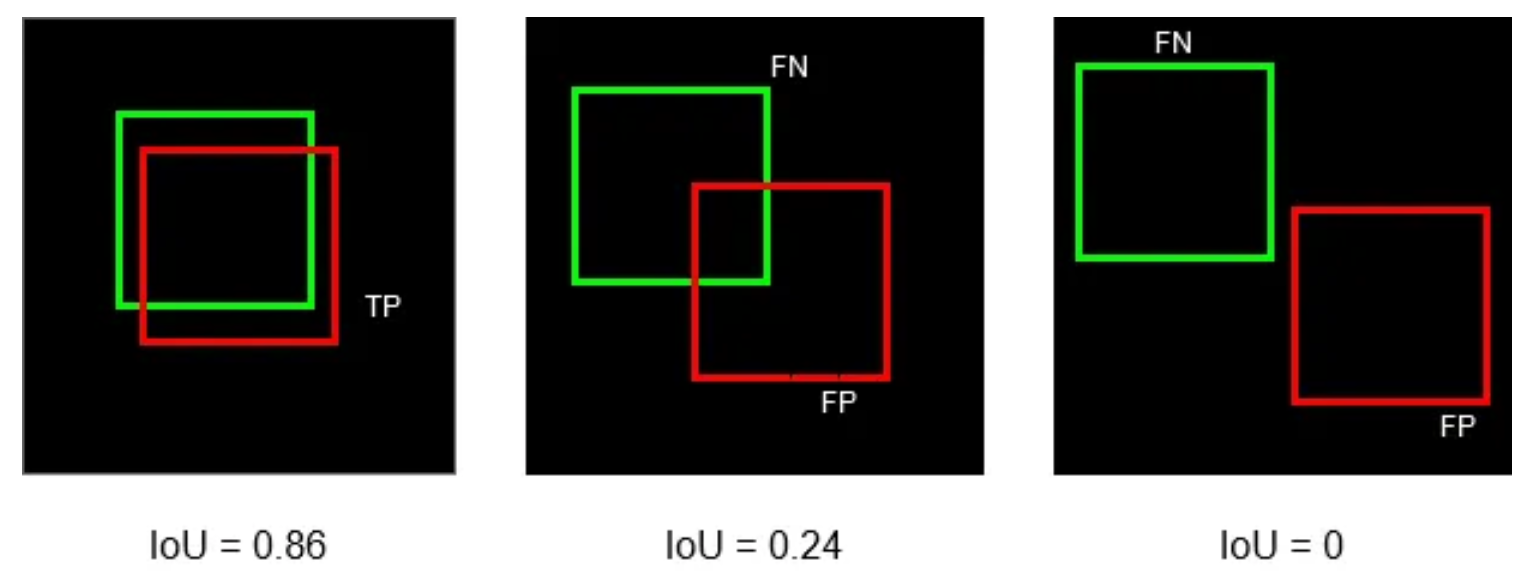
\includegraphics[width=1\textwidth]{images/05/ious.png}
    \caption{Vyhodnotenie detekcie podľa prahovej hodnoty IoU.}
    \label{img:ious}
\end{figure}

Na základe takýchto elementárnych vyhodnotení sa počíta viacero metrík. Metrika precision určuje koľko detekcií bolo skutočne pozitívnych a metrika recall určuje koľko skutočne pravdivých označení bolo odhalených skutočne pozitívnou detekciou.

Presnosť a citlivosť je okrem prahovej hodnoty IoU ovplyvnená ešte prahovou hodnotou istoty (confidence), ktorá je vypočítaná pre každú detekciu. Confidence hodnota určuje istotu modelu, že je daná detekcia správna. Model zaznačí len také detekcie, ktoré majú istotu vyššiu ako je nastavená prahová hodnota.

Závislosť medzi presnosťou a citlivosťou sa znázorňuje pomocou grafu. Obsah plochy pod krivkou je označovaný ako mAP (mean Average Precision). Výsledná hodnota mAP50 je priemer presnosti pre hodnotu prahu IoU 50\%. V prípade metriky mAP50-95 je priemer počítaný pre prah IoU od 50\% do 95\%.

V tabuľke \ref{table:test1} je každý model vyhodnotený na testovacej sade príslušnej verzie. Model M1 mal výrazne nižšie výsledky ako zvyšné dva modely. Bolo to zapríčinené tým, že pre prvý model boli ponechané aj veľmi malé reklamy, ktoré sme vyhodnotili ako nedôležité.

\begin{table}[ht]
\centering
\begin{tabular}{ |c c c c c| }
\hline
model & presnosť & citlivosť & mAP50 & mAP50-95 \\
\hline
M1  & 0.473 & 0.352	& 0.327	& 0.195 \\
M2  & 0.554	& 0.505	& 0.492	& 0.311 \\
M3  & 0.577	& 0.504	& 0.503	& 0.324 \\
\hline
\end{tabular}
\caption{Výsledky z trénovania. Modely sú označené číslom podľa verzie dát.}
\label{table:test1}
\end{table}

Pre lepšie porovnanie modelov sme pripravili spoločnú testovaciu vzorku snímok z experimentálneho merania. Vyhodnotenie modelov na testovacej vzorke v tabuľke \ref{table:test2} ukazuje, že model M3 dosahuje najlepšie výsledky v každej metrike okrem citlivosti, v ktorej vynikal druhý model. Model M1, ktorý na testovacej sade dosiahol výrazne horšie výsledky, bol napokon porovnateľný s ostatnými modelmi pri výsledkoch z testovacej vzorky, čo naznačuje, že jeho naväčšia chybovosť vychádzala z detekcií veľmi malých reklám.

\begin{table}[ht]
\centering
\begin{tabular}{ |c c c c c|  }
\hline
model & presnosť & citlivosť & mAP50 & mAP50-95 \\
\hline
M1  & 0.692	& 0.522	& 0.615	& 0.446 \\
M2  & 0.659 & \textbf{0.565} & 0.653 & 0.467 \\
M3  & \textbf{0.715} & 0.541 & \textbf{0.656} & \textbf{0.480} \\
\hline
\end{tabular}
\caption{Porovnanie tých istých modelov na spoločnej testovacej vzorke obrázkov.}
\label{table:test2}
\end{table}

Metriky boli počítané pre štandardnu prahovú hodnotu IoU (50\%) a prahová hodnota istoty bola pre každý model učrená podľa optimálnemu pomeru medzi presnosťou a citlivosťou (približne 30\%). Zmenou týchto hodnôt by sa zmenili aj výsledky metrík. Lepšie výsledky by sa dali získať optimalizáciou parametrov a rozšírením dát.

Na obrázku \ref{img:dt7} sú vykreslené detekcie z vybranej snímky. Označenie detekcie má číselnú hodnotu, ktorá určuje istotu detekcie. V tomto prípade vidíme detekciu vo väčšej vzdialenosti a detekciu reklamy s výrazným prekrytím.

\begin{figure}[ht]
    \centering
    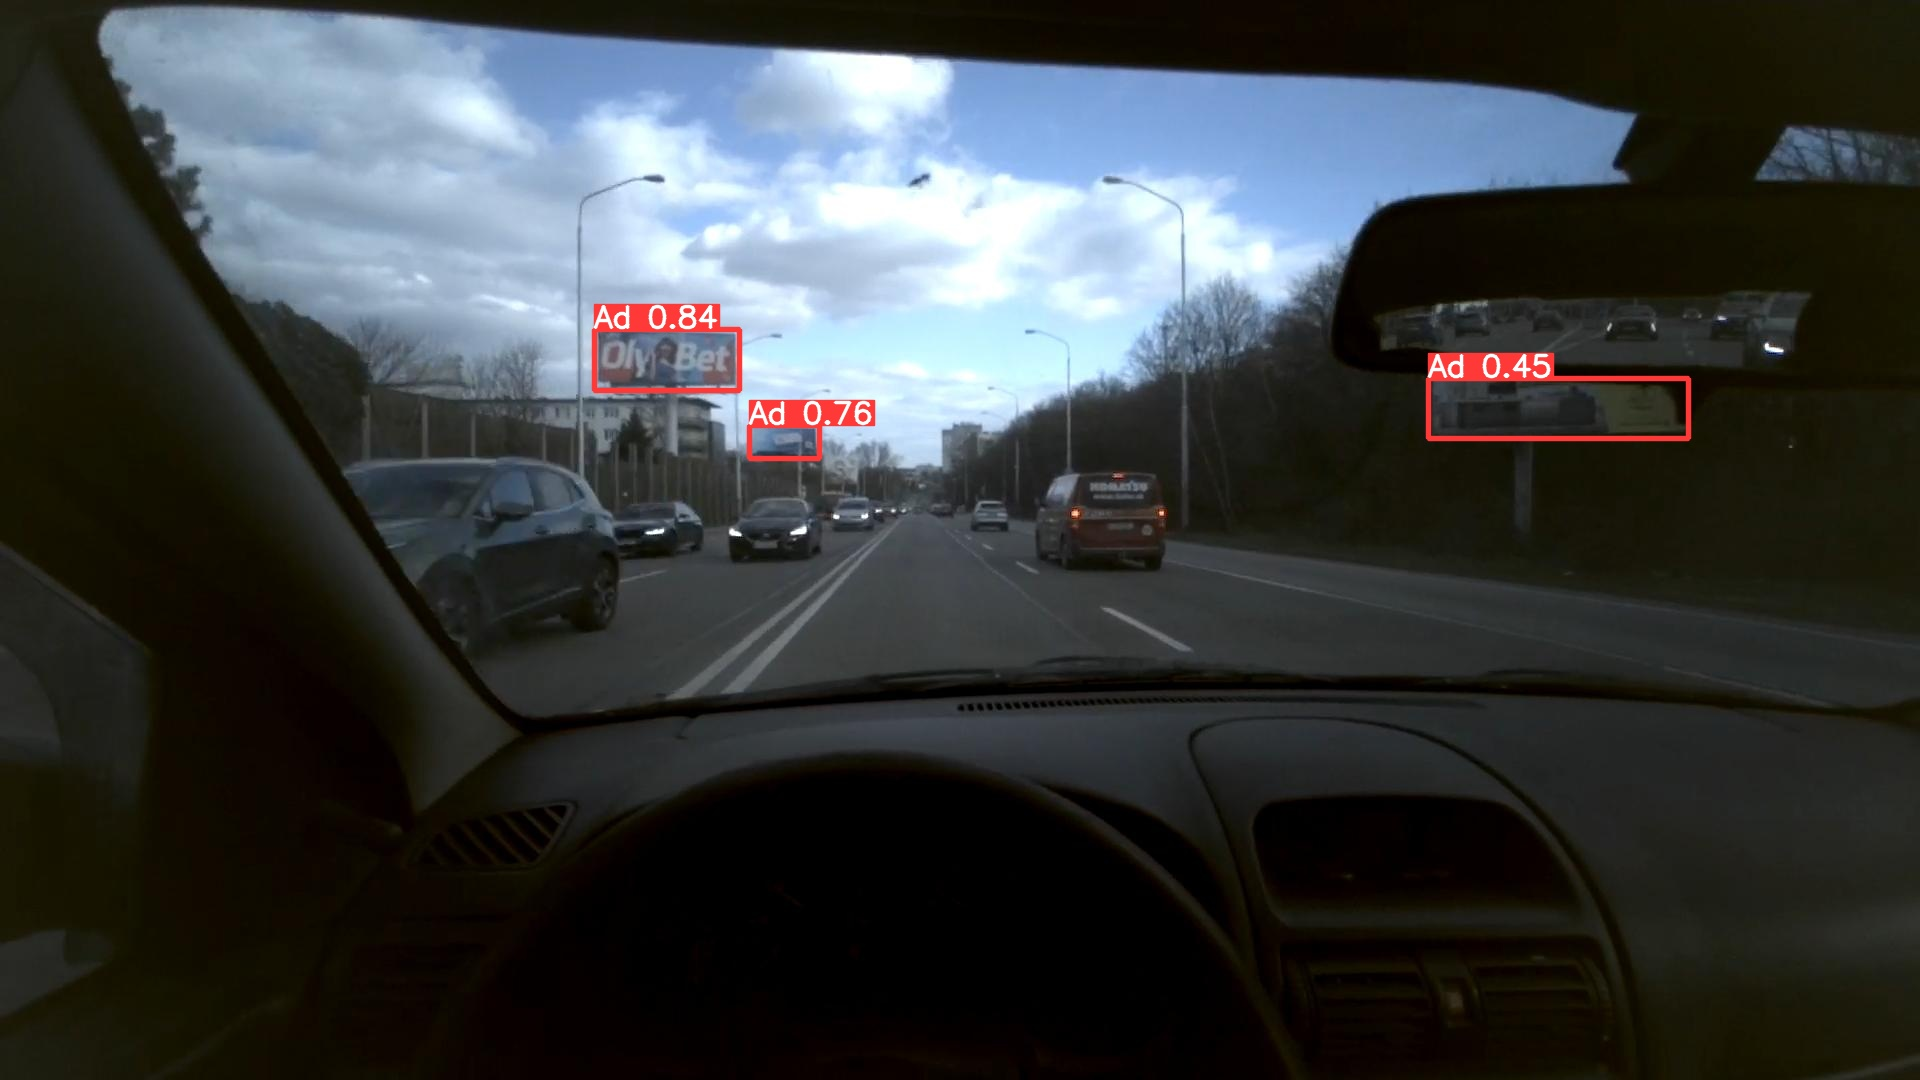
\includegraphics[width=1\textwidth]{images/05/120.jpg}
    \caption{Ukážka snímky s troma detekciami reklamy.}
    \label{img:dt7}
\end{figure}

\section{Sledovanie reklám}

Na vyhodnotenie sledovania objektov, existuje viacero zaužívaných metrík. Rozhodli sme sa použiť metriku so skratkou HOTA (Higher Order Tracking Accuracy) \cite{hota}, ktorá sa kladá z menších častí, podľa ktorých sa dajú vyhodnotiť tri aspekty sledovania: lokalizácia, detekcia a asociácia.

Lokalizácia a detekcia sa meria rovnako ako pri testovaní detektorov. Asociácia meria ako dobre sa podarilo spojiť detekciu s referenciou. Podobne ako pri detekcii môžu nastať tri stavy, ktoré určujú správnosť asociácie:

\begin{itemize}
  \item skutočne pozitívna asociácia (true positive association, TP)
  \item falošne pozitívna asociácia (false positive association, FP)
  \item falošne negativna asociácia (false negative association, FN)
\end{itemize}

% https://jonathonluiten.medium.com/how-to-evaluate-tracking-with-the-hota-metrics-754036d183e1
% https://arxiv.org/pdf/2009.07736.pdf

Obrázok \ref{cite:usecase} vysvetľuje koncepty TPA, FPA a FNA na objekte, ktorý je označený v červenom štvorci. Zelená farba označuje stav TPA, v ktorom je predikovaná referencia rovnaká so skutočnou referenciou objektu. Žltá farba označuje FPA, ktorá je v prvom prípade zapríčinená FP detekciou a v druhom prípade tým, že asociácia vstupuje to trajektórie iného objektu. Hnedá farba označuje FNA v prípade, kde sa nepodarilo zachytiť skutočnú časť trajektórie.

\begin{figure}[ht]
    \centering
    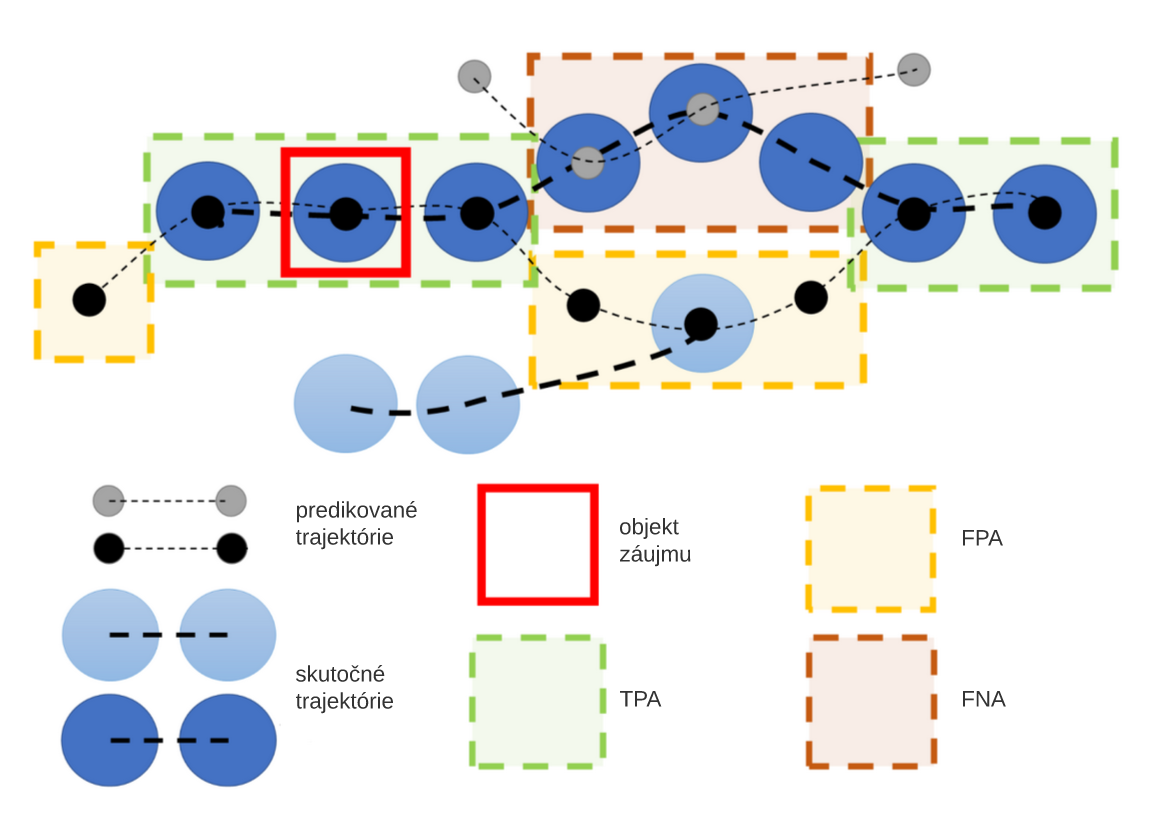
\includegraphics[width=0.7\textwidth]{images/05/usecase.png}
    \caption{Vizualizácia všetkých možností, ktoré môžu vzniknúť pri sledovaní \cite{hota}.}
    \label{img:usecase}
\end{figure}

Geometrickým priemerom detekcie a asociácie je vypočítaná hodnota HOTA. Táto formulácia zabezpečuje, že detekcia aj asociácia sú na rozdiel od mnohých iných metrík sledovania rovnomerne vyvážené a že konečné skóre je niekde medzi nimi.

Každá sledovacia metóda bola spustená viackrát s rôznou konfiguráciou. Najlepšie výsledky pre každú metódu sú zapísané v tabuľke \ref{table:hota1}. Skratky DetPr, DetRe, DetA značia presnosť, citlivosť a celkovú úspešnosť detekcie a podobne to platí pre asociáciu.
\\
\begin{table}[ht]
\centering
\begin{tabular}{|l l l l l l l l l|}
 \hline
metóda & HOTA & DetPr & DetRe & DetA & AssPr & AssRe & AssA & Loc \\ [0.5ex]
 \hline
OC-SORT & 36.8  &  39.5  &  34.3  &  53.2  &   58.2  &  36.3   &  \textbf{85.1}  &  89.1 \\ [0.1ex]
DeepOC-SORT & 35.8 &   38.9  &  33.0  &  54.4  &  55.6  &  34.8  &  84.7  &  89.1 \\ [0.1ex]
StrongSORT & \textbf{38.5}  &  \textbf{41.4}  &  \textbf{35.8}  &  \textbf{54.6} &   60.6   &   \textbf{42.7}   & 72.9   & 88.7 \\ [0.1ex]
BotSORT & 37.0  &  39.5  &  34.7  &  53.0  &  58.4  &  37.5 &   82.6  &  \textbf{89.2} \\ [0.1ex]
ByteTrack & 32.6  &  36.4  &  29.3  &  44.4  &  \textbf{62.8}  &  30.5  &  84.7  &  86.6 \\ [0.1ex]
 \hline
\end{tabular}
\caption{Porovnanie výsledkov piatich sledovacích metód.}
\label{table:hota1}
\end{table}

Metóda StrongSORT obstála najlepšie v celkovej metrike HOTA a vo väčšine zvyšných metrík. V prípade presnosti asociácie bola najlepšia metóda ByteTack, ktorá však nadobúdala najnižšie hodnoty takmer pre všetky ostatné metriky. Na vypočítavanie významnosti reklám bolo najlepšie použiť metódu StrongSORT, ktorá dosiahla najvyšší počet detekcií s relatívne dobrým priraďovaním referencií.

\section{Významnosť reklám}

Na zvolenej trase bolo dokopy nájdených 145 reklám. V tabuľke \ref{table:cat} je pre každú kategóriu zapísané časové rozmedzie (korešpondujúce počtu snímok s prienikom), počet reklám v príslušnej kategórie a priemerný počet vodičov, ktorí sa pozreli na reklamu. Zaradenie do kategórií bolo počítané z výsledkov pomocného modelu a sledovacej metódy StrongSORT.

\begin{table}[ht]
\centering
\begin{tabular}{|l l c c|}
 \hline
 kategória &	rozmedzie &	počet reklám &	počet vodičov \\ [0.5ex]
 \hline
slabá &	0 ms &	45 &	- \\ [0.1ex]
nízka &	1-249 ms &	79 &	3 \\ [0.1ex]
stredná &	250-499 ms &	17 &	3 \\ [0.1ex]
vysoká &	500+ ms &	4 &	4 \\ [0.1ex]
 \hline
\end{tabular}
\caption{TODO, výsledky 5.}
\label{table:cat}
\end{table}

Priemerne sa na jednu reklamu pozreli traja vodiči a 45 reklám sa nepozrel ani jeden vodič. Len v dvoch prípadoch sa stalo, že si reklamu všimli všetci vodiči. Naopak 34 krát sa stalo, že významnosť reklamy bola určená len na základe jedného vodiča, ktorý sa na ňu pozrel. V grafe \ref{img:chart} je znázornená distribúcia reklám do kategórií, ktorá je veľmi nevyvážená, hlavne pre vysokú významnosť.

\begin{figure}[ht]
    \centering
    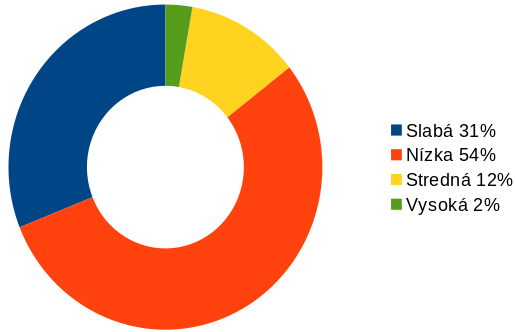
\includegraphics[width=0.6\textwidth]{images/05/chart.png}
    \caption{Distribúcia reklám do kategórií.}
    \label{img:chart}
\end{figure}

\section{Klasifikácia reklám}

Na klasifikáciu bolo vypočítaných niekoľko príznakov, z ktorých by sa dalo vyvodiť niekoľko daľších štatistických údajov. Najzaujímavejším príznakom je však mapa význačností počítaná z videa. Presnosť 69

V niektorých prípadoch, ako napríklad na obrázku \ref{img:salmap}, je vidieť, že mapa význačnosti jasne zachytí oblasť s reklamou.

\begin{figure}[H]
    \centering
    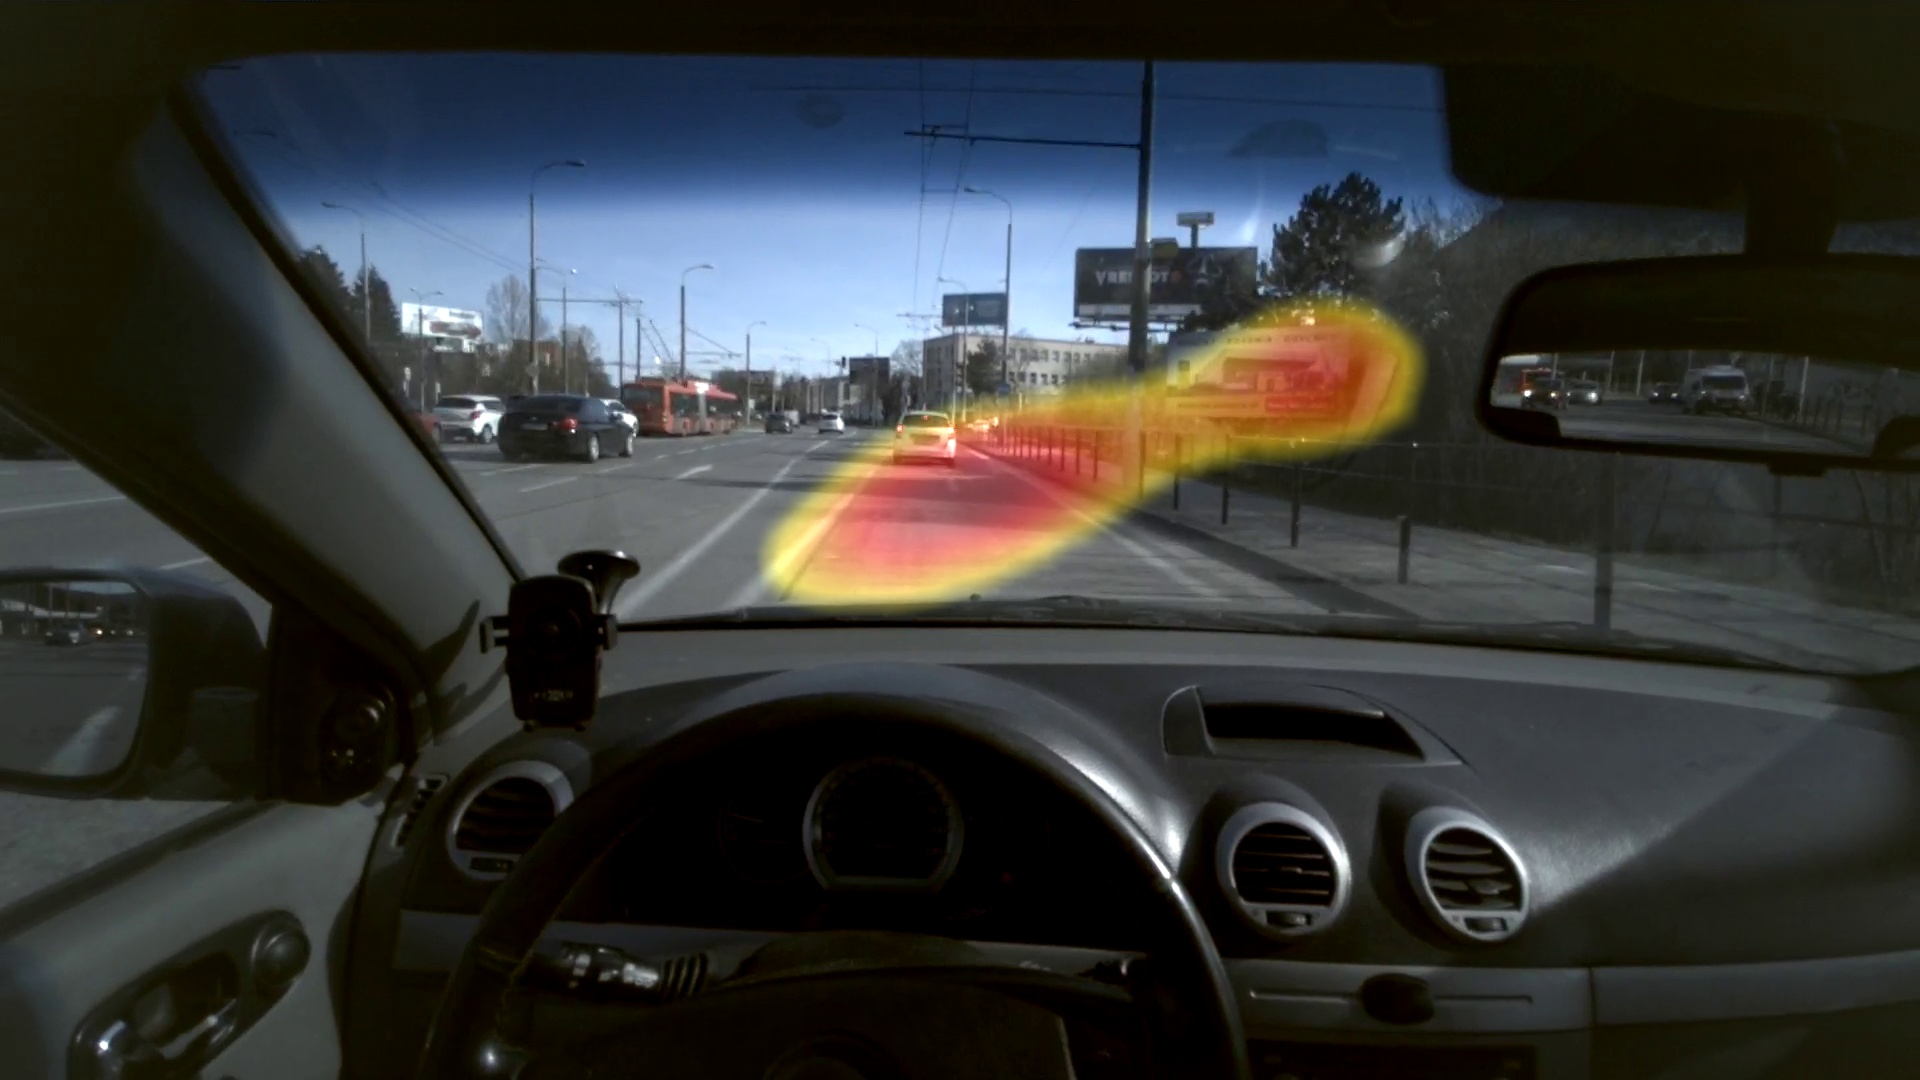
\includegraphics[width=1\textwidth]{images/05/sal_frame.jpg}
    \caption{Ukážka prekrytia mapy význačnosti so snímkou z experimentu.}
    \label{img:salmap}
\end{figure}

ahoj

\begin{figure}[ht]
    \centering
    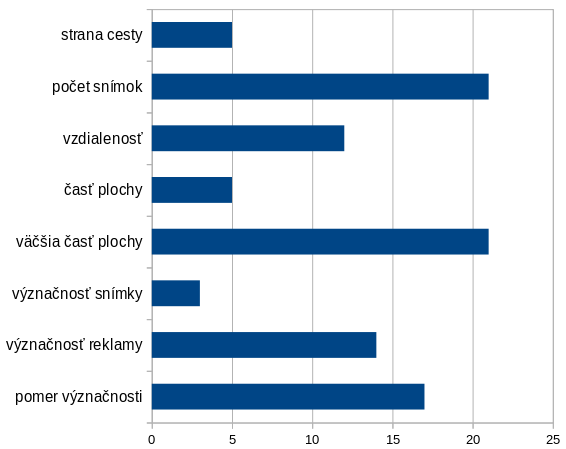
\includegraphics[width=0.6\textwidth]{images/05/chart2.png}
    \caption{Dôležitosť príznakov.}
    \label{img:road}
\end{figure}

%Na získanie čo najlepších výsledkov sme vyskúšali natrénovať niekoľko stromov.
%
%Best hyper parameters: {'n_estimators': 130, 'min_samples_leaf': 3, 'max_leaf_nodes': 10, 'max_features': 'sqrt', 'max_depth': 3}
%
%n_estimator, The number of trees in the forest
%
%max_leaf_node, Grow trees with max_leaf_nodes in best-first fashion. Best nodes are defined as relative reduction in impurity. If None then unlimited number of leaf nodes.



%Spojením všetkých príznakov... TODO

\begin{figure}[ht]
    \centering
    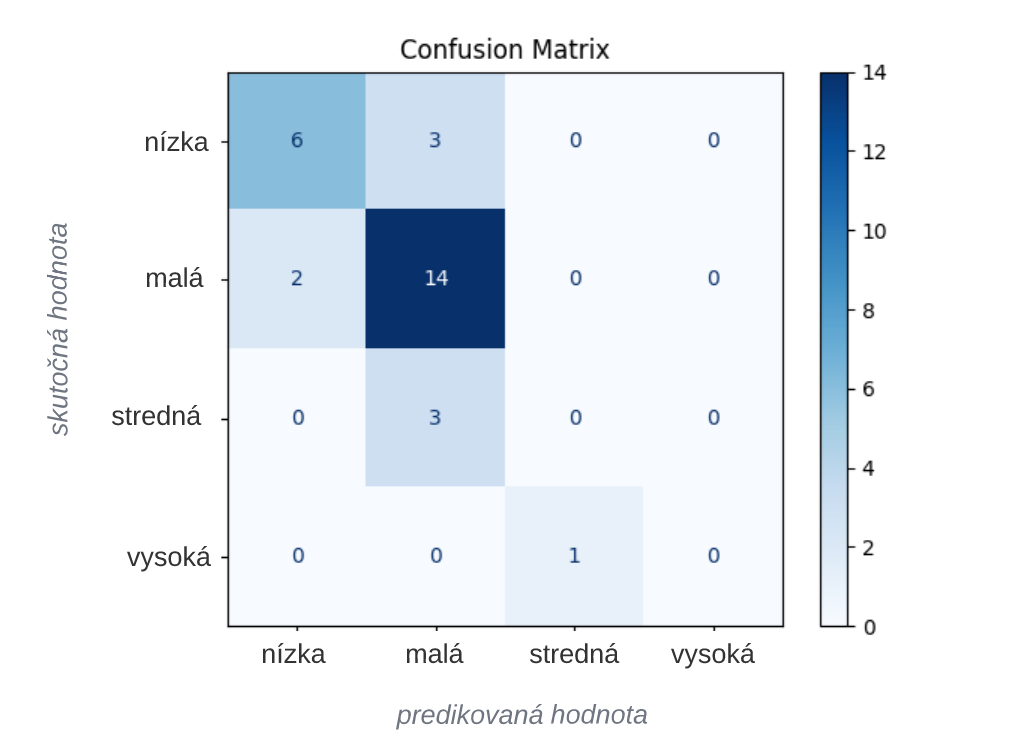
\includegraphics[width=0.5\textwidth]{images/05/v3.png}
    \caption{Výsledky klasifikácie s použitím RFC.}
    \label{img:matrix}
\end{figure}

%Jeden z rozhodovacích stromov je generovaný na obrázku \ref{img:tree}. Údaje rozdeľuje na základe niekoľkých funkcií vrátane „strana“, „výraznosť masky“, „vzdialenosť“ a „pomer_väčšej_veľkosti“. Hodnoty v uzloch predstavujú rozdelenie tried v zodpovedajúcej podmnožine údajov. Strom má štyri úrovne hĺbky a maximálnu hĺbku stromu je možné ovládať ako parameter algoritmu. Farba uzlov predstavuje distribúciu tried v podmnožine údajov.

\begin{figure}[ht]
    \centering
    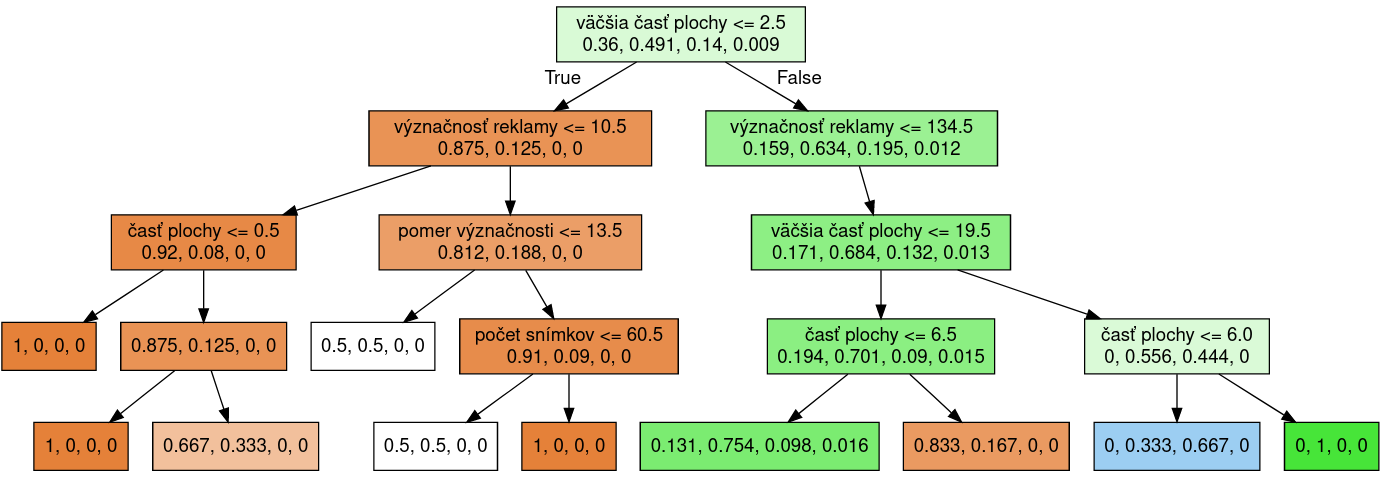
\includegraphics[width=1\textwidth]{images/05/tree.png}
    \caption{Dôležitosť príznakov.}
    \label{img:tree}
\end{figure}